\documentclass[a4paper,11pt,fleqn]{article}%fleqn pour aligner les equations à gauche
\usepackage{graphicx}
\usepackage[utf8]{inputenc}  
\usepackage[T1]{fontenc}
\usepackage{lscape}
\usepackage{pifont}%utilier symboles ding
\usepackage{subcaption}

\usepackage{tgheros,textcomp}%Police Arial
\renewcommand{\familydefault}{\sfdefault}

%\setlength{\mathindent}{0pt}%indentation dans math = 0

\usepackage[top = 1cm, bottom = 2cm, left = 1cm, right = 1cm]{geometry}
\usepackage{titlesec}
%\setcounter{secnumdepth}{4}
\usepackage{xcolor}
\usepackage{amssymb} %double flèche de réaction
\usepackage{mathrsfs}%farraday
\usepackage{xtab}%tableau sur plusieurs pages
\usepackage{esvect}%grands vecteurs

\usepackage[version=4]{mhchem} %equations chimiques

\usepackage{array}
\usepackage{chemfig}
\usepackage{multirow}
%\usepackage{sectsty}

\usepackage{caption}
\usepackage{adjustbox}
\usepackage[labelformat=simple]{subfig}
\usepackage{float}


\usepackage{amsmath}
\usepackage{amssymb}
\usepackage[cal=boondoxo]{mathalfa} 
\usepackage{enumitem}
\usepackage{lastpage}
\usepackage{tcolorbox}
\usepackage{siunitx}
\usepackage[european, straightvoltages, RPvoltages]{circuitikz}
\usepackage{tikz}
\usetikzlibrary{shapes.geometric}
\usetikzlibrary{calc}
\usetikzlibrary{automata,positioning}
\usepackage{multicol}
\usepackage{eqnarray}
\usepackage{tabularx,colortbl}%colorer fond cellules

\sisetup{
	detect-all,
	output-decimal-marker={,},
	group-minimum-digits = 3,
	group-separator={~},
	number-unit-separator={~},
	inter-unit-product={~}
} %setup pour SIunitx

\usepackage{listings}%pour insérer le code python
\definecolor{codegreen}{rgb}{0,0.6,0}
\definecolor{codegray}{rgb}{0.5,0.5,0.5}
\definecolor{codepurple}{rgb}{0.58,0,0.82}
\definecolor{backcolour}{rgb}{0.95,0.95,0.92}

\lstdefinestyle{mystyle}{
    backgroundcolor=\color{backcolour},   
    commentstyle=\color{codegreen},
    keywordstyle=\color{magenta},
    numberstyle=\tiny\color{codegray},
    stringstyle=\color{codepurple},
    basicstyle=\ttfamily\footnotesize,
    breakatwhitespace=false,         
    breaklines=true,                 
    captionpos=b,                    
    keepspaces=true,                 
    numbers=left,                    
    numbersep=5pt,                  
    showspaces=false,                
    showstringspaces=false,
    showtabs=false,                  
    tabsize=2
}

\lstset{style=mystyle}

\titleformat{\section}
{
\vspace{.8ex}%
\normalfont \bfseries \large}
{\thesection.}{.5em}{\bfseries}

\renewcommand{\thesection}{\arabic{section}}
\titlespacing{\section}{0pt}{1em}{.5em}
\renewcommand{\thesubsection}{\hspace{1cm}\alph{subsection}.}
\renewcommand\thesubfigure{\textbf{Document \arabic{subfigure} :}}

\title{\vspace{-1cm}\large 
	\begin{tabular}{|>{\centering}m{5cm}|>{\centering}m{8cm}|>{\centering\arraybackslash}m{4cm}|}
		\hline
		Activité 2 & \textbf{\textsc{La forme de la Terre dans l'Antiquité}} &  Chapitre 4 \\
		\hline
\end{tabular}}
\date{}

\newpagestyle{mystyle}{%
	\setfoot{ROSALIE}{\thepage\,$|$\,\pageref{LastPage}}{}
}
\renewpagestyle{plain}{%
	\setfoot{ROSALIE}{\thepage\,$|$\,\pageref{LastPage}}{}
}

\pagestyle{mystyle}

\newenvironment{itemize*}%
{\begin{itemize}[label=$-$,labelindent=0pt, leftmargin=*,topsep=0pt]%
		\setlength{\itemsep}{0pt}%
		\setlength{\parskip}{0pt}}%
	{\end{itemize}}

\newenvironment{itemize**}%
{\begin{itemize}[label=,labelindent=0pt, leftmargin=*,topsep=0pt]%
		\setlength{\itemsep}{0pt}%
		\setlength{\parskip}{0pt}}%
	{\end{itemize}}

\renewcommand{\arraystretch}{1.5}

\begin{document}
\maketitle
\vspace{-2cm}

Dès l'Antiquité, les penseurs s'interrogent sur la forme de la planète sur laquelle ils vivent. Les courants de pensée, philosophiques puis scientifiques, les amènent à adopter différentes représentations de la Terre.\\
\textbf{Comment les savants grecs sont-ils parvenus à estimer que la Terre était une sphère d'un rayon d'environ \SI{6400}{km} ?}

\noindent\colorbox{blue!10}{\begin{minipage}[t][9.5cm][t]{.48\linewidth}
		\textcolor{purple!30!blue}{\textbf{Document 1 : Expliquer l'Univers}}\\
		C'est à la fin du {7}$^e$ siècle de notre ère que naît la philosophie grecque. Les premiers philosophes, également mathématiciens, cherchent à expliquer la création de l'Univers de manière rationnelle, rompant ainsi avec une vision liée à l'intervention des dieux dans sa genèse.\\
		En Ionie (actuellement Turquie), le philosophe et savant grec Thalès de Milet (625-547 av. J.-C.) fonde son école après avoir été formé à l'astronomie en Égypte. On lui attribue l'idée d'une Terre en forme de disque flottant sur un océan infini.\\
		Sur les côtes méridionales de la Grande-Grèce, le philosophe grec Pythagore (580-495 av. J.-C.) et les pythagoriciens interprètent l'Univers à travers le prisme des mathématiques, sciences des proportions et de l'harmonie.
\end{minipage}}
\colorbox{blue!10}{\begin{minipage}[t][9.5cm][t]{.5\linewidth}
		\textcolor{purple!30!blue}{\textbf{Document 2 : L'évolution des représentations de la Terre}}\\
		Pythagore et ses disciples imaginent la Terre sous la forme d'une sphère afin de répondre à une exigence de symétrie parfaite. En effet, ils observent la course des étoiles se déplaçant sur une demi-sphère cosmique, et si le ciel est une sphère, la Terre doit l'être aussi.\\
		Les représentations de la Terre ressemblent encore à une construction mystique plutôt qu'au modèle d'une théorie scientifique.\\
		Mais l'Univers demeure expliqué en se fondant sur une base unique : l'eau pour l'école ionienne, les nombres pour l'école de Pythagore, et même l'idée du Bien pour l'Académie, l'école athénienne du philosophe grec Platon (428-348 av. J.-C.).\\
		Il faudra attendre son disciple Aristote (384-332 av. J.-C.) qui, tout en conservant l'idée de rigueur insufflée par son maître, rompt avec cette vision purement philosophique, et place l'observation et la démonstration au c\oe ur de sa réflexion.
\end{minipage}}
        \begin{center}
			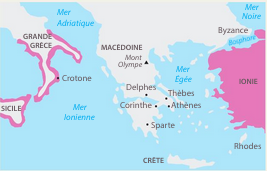
\includegraphics[width=.4\linewidth]{Ressources/1ES_C4_AE2_Fig3.png}
		\end{center}

\noindent \begin{minipage}{.5\linewidth}
    \begin{center}\textcolor{orange}{\textbf{Vocabulaire}}\end{center}
\textcolor{orange}{\textbf{Gnomon : }} Tige verticale plantée dans le sol, utilisée dans l'Antiquité, et sont l'ombre permet de déterminer l'orientation des rayons du Soleil.\\
\textcolor{orange}{\textbf{Stade : }} Unité de longueur de référence dans l'Antiquité, équivalant à \SI{157,7}{m}.\\
\textcolor{orange}{\textbf{Mystique :}} Adjectif qui qualifie des pratiques liées aux divinités, aux croyances.\\
\textcolor{orange}{\textbf{Septentrional :}} qui appartient aux régions du Nord
\end{minipage}
\begin{minipage}{.5\linewidth}
\begin{center}\textcolor{red}{\textbf{Questions}} \end{center}
\begin{enumerate}
	\item Quel mathématicien commence à imaginer que la Terre est de forme sphérique ? Comment l'explique-t-il ?
	\item Pourquoi parle-t-on de "rupture" dans la démarche d'Aristote ?
	\item Pourquoi Eratosthène considère-t-il les rayons du Soleil comme parallèles entre eux ? Que peut-on en déduire quant aux angles $\alpha$ et $\beta$ ?
	\item Calculer la distance d'Alexandrie à Syène en mètres.
	\item Retrouver le raisonnement géométrique qu'Eratosthène a mené pour estimer que la circonférence de la Terre est proche de \SI{40000}{km}. En déduire le rayon de la Terre.
\end{enumerate}
\end{minipage}


\noindent \colorbox{blue!10}{\begin{minipage}{.7\linewidth}
		\textcolor{purple!30!blue}{\textbf{Document 3 : Du Ciel}}\\
		Dans le traité \emph{Du ciel} (350 av. J.-C.), Aristote explique les raisons pour lesquelles la Terre est de forme sphérique.\\
		"Dans les éclipses de Lune, la ligne qui limite l'ombre est toujours une ligne incurvée. Puisque l'éclipse est due à l'interposition de la Terre entre la Lune et le Soleil, c'est la forme de la surface de la Terre, sphérique, qui produit cette ligne courbe. De plus, la manière dont les astres nous apparaissent ne prouve pas seulement que la Terre est ronde, mais aussi que son étendue est assez petite. En effectuant un déplacement minimale vers le Sud ou vers le Nord, nous voyons se modifier le cercle d'horizon. Les astres au-dessus de nous changent considérablement, et ce ne sont pas les mêmes qui brillent dans le ciel quand on va vers le Nord et quand on va vers le Sud. certains astres visibles en Égypte ou vers Chypre sont invisibles dans dans les régions septentrionales. Par ailleurs, les astres qui, dans les régions septentrionales sont visibles à tout instant, connaissent un coucher dans les pays cités plus haut. Tout cela ne montre pas seulement que la Terre est ronde, mais encore qu'elle a la forme d'une sphère de modeste dimension."
\end{minipage}
\begin{minipage}{.3\linewidth}
		\centering
		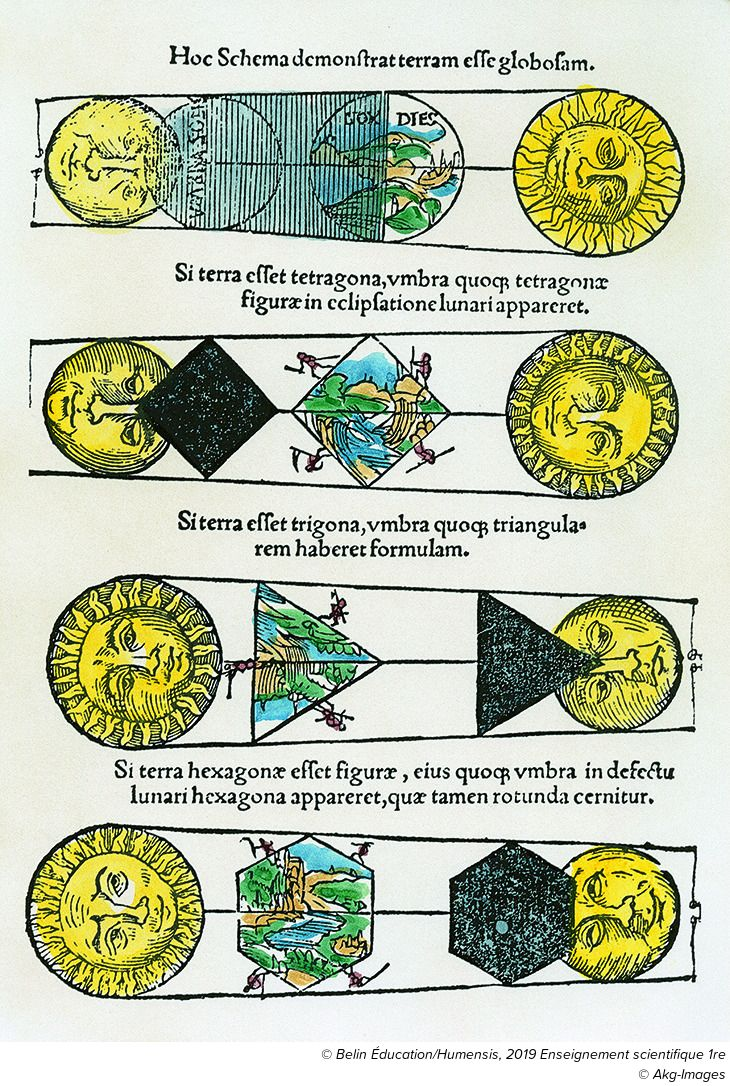
\includegraphics[width=\linewidth]{Ressources/1ES_C4_AE2.jpg}
\end{minipage}}

\noindent \colorbox{blue!10}{\begin{minipage}{.7\linewidth}
		\textcolor{purple!30!blue}{\textbf{Document 4 : La mesure de la circonférence de la Terre}}\\
		À la fin du 2$^e$ siècle avant J.-C, le modèle d'une Terre sphérique est accepté dans les milieux intellectuels grecs et la question de ses dimensions se pose.\\
		L'astronome et géographe grec Eratosthène (276-194 av. J.-C.) dirige alors la grande bibliothèque d'Alexandrie en Égypte. Il y lit que le jour du solstice d'été, à midi à Syène, actuelle ville d'Assouan en Égypte, le Soleil éclaire le fond d'un puit. Les rayons lumineux arrivent donc en ce lieu à la verticale du sol : une personne debout à Syène en ce jour précis ne verra pas son ombre au sol. Eratosthène sait alors comment déterminer la circonférence de la Terre car il connaît la proportionnalité liant la longueur de l'arc de cercle \{Alexandrie-Syène\} à l'angle au centre de la Terre qui l'intercepte. Avec la formule de la longueur d'un cercle, il peut en déduire le rayon de la Terre.\\
  
		\emph{L'expérience d'Eratosthène}\\
		Eratosthène considère que le Soleil est très éloigné de la Terre et que, de fait, ses rayons peuvent être considérés comme parallèles entre eux. Il plante verticalement un gnomon dans le sol afin d'en observer l'ombre et ainsi calculer l'angle formé entre le gnomon et son ombre. L'ensemble formant un triangle rectangle, il applique les règles de trigonométrie classiques pour calculer la valeur de l'angle : $\beta$ = \SI{7.2}{\degree}.
\end{minipage}
\begin{minipage}{.3\linewidth}
	\centering
	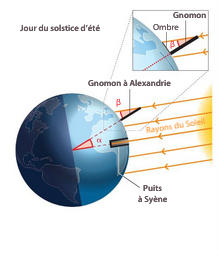
\includegraphics[width=\linewidth]{Ressources/1ES_C4_AE2_Fig2.png}
\end{minipage}}

\vspace{.25cm}
\noindent \colorbox{blue!10}{\begin{minipage}{.5\linewidth}
		\textcolor{purple!30!blue}{\textbf{Document 5 : La distance Alexandrie-Syène}}\\
		Nous ne disposons aujourd'hui d'aucun écrit d'Eratosthène. Aussi, plusieurs idées circulent sur la manière dont il a mesuré la distance Alexandrie-Syène.\\
		La plus courante indique qu'il se serait base sur le fait d'un chameau met environ 5 jours pour aller d'Alexandrie à Syène et, qu'en un jour, le chameau parcourt une distance de 100 stades : la distance entre le deux villes est donc d'environ 500 stades.
\end{minipage}
\begin{minipage}{.5\linewidth}
	\textcolor{orange}{\begin{center}\textbf{Maths}\end{center}}
	\begin{itemize}[topsep=0pt]
		\item Si les droites ($d_1$) et ($d_2$) sont parallèles, les angles alternes-internes sont égaux.\\
		\begin{center}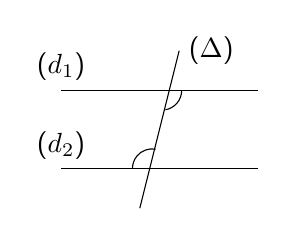
\begin{tikzpicture}[scale=.5]
			\draw (0,0)--(5,0);
			\draw (0,-2)--(5,-2);
			\draw (3,1)--(2,-3);
			
			\node[above] at (0,0) {($d_1$)};
			\node[above] at (0,-2) {($d_2$)};
			\node[right] at (3,1) {($\Delta$)};
			
			\draw (2.65,-.5) arc(-80:0:.5);
			\draw (2.4,-1.5) arc(80:180:.5);
		\end{tikzpicture}
        \end{center}
		\item La longueur du pourtour $P$ d'un cercle de rayon $r$ est définie par la relation :
		$$P = 2 \times \pi \times r$$
	\end{itemize}
\end{minipage}}



\end{document}